\documentclass[cs4size,a4paper,adobefonts,openany]{ctexbook}
\usepackage[colorlinks=true,linkcolor=black]{hyperref}
\usepackage{indentfirst}
\usepackage[a4paper,left=2.5cm,right=2.5cm,bottom=2.5cm,top=2.5cm]{geometry}
\usepackage{amsmath,amsthm,amssymb}
\usepackage{fontspec}
\setmainfont{Palatino}
\pagestyle{plain}
\punctstyle{kaiming}
\usepackage{unicode-math}
\setmathfont{Asana Math}
\usepackage{color}

\newtheorem{defn}{定义}
\newtheorem{thm}{定理}
\newcommand{\pname}[1]{\underline{#1}}
\numberwithin{equation}{section}
\CTEXsetup[number=\thechapter]{chapter}

\newcommand{\starSym}{\ {\color{red}{$\ast$}}\ }
\begin{document}
\title{\bfseries The Symmetries of Things 的学习笔记}
\author{王盛颐}
\date{}
\maketitle
\setcounter{page}{1}
\chapter{Symmetries}

这章主要介绍一种描述对称的记号,最早是由 Murray MacBeath 提出来的。

\section{Kaleidoscopes}
最简单的一个记号就只是一个 \starSym。一个 \starSym 表示一个\pname{镜像}
(mirror) 对称或者叫\pname{万花筒} (kaleidoscopic) 对称。单独的一个
\starSym 表示图像没有其它对称性了,如图 \ref{pic:star} 所示的那样,只有
一个镜像对称的对称轴。
\begin{figure}[htbp]
\label{pic:star}
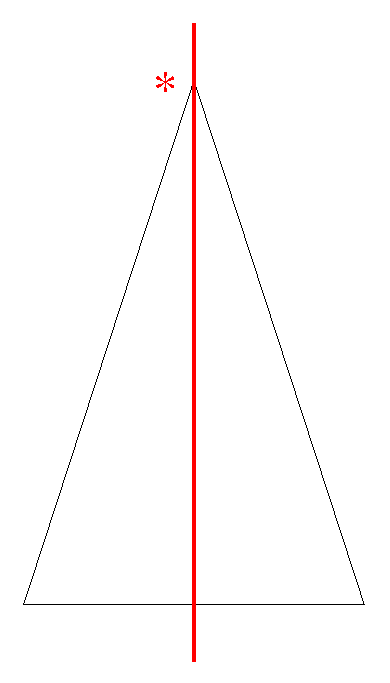
\includegraphics[width=.2\textwidth]{images/star}
\end{figure}

\end{document}
